\documentclass[11pt,a4paper]{report}

\usepackage[utf8]{inputenc}
\usepackage[T1]{fontenc}
\usepackage[italian]{babel}
\usepackage{lmodern}
\usepackage{geometry}
\geometry{margin=2.5cm}
\usepackage{setspace}
\onehalfspacing
\usepackage{graphicx}
\usepackage{float}
\usepackage{booktabs}
\usepackage{caption}
\usepackage{subcaption}
\usepackage{amsmath,amssymb}
\usepackage{siunitx}
\usepackage{xcolor}
\usepackage{enumitem}
\usepackage{hyperref}
\usepackage{listings}
\usepackage{tcolorbox}
\usepackage{longtable}
\usepackage{array}
\usepackage{multirow}
\usepackage{url}

\hypersetup{colorlinks=true,linkcolor=blue,citecolor=blue,urlcolor=blue}
\tcbset{colback=gray!5,colframe=gray!50!black,boxrule=0.5pt,arc=1mm}
\lstset{
  basicstyle=\ttfamily\small,
  breaklines=true,
  frame=tb,
  numbers=left,
  numberstyle=\tiny,
  keywordstyle=\color{blue!70!black},
  commentstyle=\color{gray!80!black},
  stringstyle=\color{teal!70!black}
}
\graphicspath{{selected_figures/}}

\newcommand{\dataset}{\texttt{Flickr8k}}
\newcommand{\bos}{\texttt{<bos>}}
\newcommand{\eos}{\texttt{<eos>}}
\newcommand{\pad}{\texttt{<pad>}}
\newcommand{\unk}{\texttt{<unk>}}

\begin{document}

\begin{titlepage}
  \centering

  {\Large \textbf{Università degli Studi di Parma} \\[0.3em]
  \textbf{Corso di Laurea in Ingegneria Informatica} \\[0.3em]
  Curriculum: \textbf{Intelligenza Artificiale} \\[2em]}

  {\Huge \textbf{Image Captioning con CNN--LSTM su Flickr8k}}\\[0.8em]
  {\Large Report accademico revisionato e riallineato ai risultati sperimentali reali}\\[1.5em]

  \rule{\linewidth}{0.4pt}\\[0.8em]
  \textbf{Obiettivo del progetto.}
  Il presente elaborato documenta in modo sistematico lo sviluppo di un sistema di \emph{image captioning} basato su architettura CNN--LSTM, con particolare attenzione alla coerenza tra implementazione, protocollo sperimentale e risultati effettivamente ottenuti. Il documento non si limita a descrivere il funzionamento teorico del modello, ma ricostruisce l'intera pipeline realizzata nel repository: preparazione dei dati, costruzione del vocabolario, addestramento, studio di ablation e analisi qualitativa delle didascalie generate.\\[0.8em]
  \rule{\linewidth}{0.4pt}\\[3em]

  \begin{tabular}{ll}
  Studente: & Giuseppe Dimonte \\
  Matricola: & 367431 \\
  Docente: & Prof. Andrea Prati \\
  Corso: & Deep Learning e Modelli Generativi \\
  Anno accademico: & 2025/26 \\
  \end{tabular}

  \vfill
  {\large \today}
\end{titlepage}

\tableofcontents
\clearpage

\begin{abstract}
Il progetto affronta il task di \emph{image captioning}, ovvero la generazione automatica di una descrizione testuale a partire dal contenuto visivo di un'immagine. Il lavoro è stato sviluppato sul dataset pubblico \dataset{}, scelto per la sua diffusione come benchmark di piccola scala nei problemi di visione-linguaggio, ed è stato implementato in PyTorch mediante una pipeline \emph{image-to-sequence} costituita da un encoder convoluzionale pre-addestrato e da un decoder LSTM. Rispetto a una semplice relazione descrittiva, il presente documento assume una prospettiva più rigorosa: le scelte architetturali sono motivate rispetto al vincolo del dataset, il protocollo sperimentale è ricostruito a partire dai file di configurazione e dai log reali, e i risultati quantitativi vengono letti criticamente alla luce delle diverse varianti addestrate.

La campagna sperimentale ha incluso una baseline e tre ablation controllate: rimozione dello scheduled sampling, rimozione del label smoothing e attivazione del fine-tuning della CNN. I risultati, valutati tramite punteggi BLEU e analisi qualitativa delle caption, mostrano che la configurazione migliore è quella con fine-tuning della componente convoluzionale, che raggiunge un BLEU-4 pari a 0.0649. Al contrario, la rimozione dello scheduled sampling e del label smoothing determina un peggioramento coerente su tutte le metriche principali. La relazione discute inoltre i limiti del modello, le discrepanze tra loss e qualità linguistica e le implicazioni metodologiche derivanti dall'addestramento in ambiente CPU-only.
\end{abstract}

\chapter{Introduzione}

\section{Perché l'image captioning è un problema significativo}

L'\emph{image captioning} rappresenta uno dei problemi più interessanti dell'intelligenza artificiale contemporanea perché richiede la cooperazione tra due competenze normalmente studiate separatamente: la comprensione del contenuto visivo e la generazione di linguaggio naturale. Un sistema di captioning non deve infatti soltanto riconoscere oggetti presenti in un'immagine, ma deve selezionare le informazioni rilevanti, organizzarle in una struttura sintatticamente plausibile e produrre una frase breve ma semanticamente coerente. In questo senso, il problema è più complesso di una semplice classificazione di immagini e più vincolato, ma anche più interpretabile, rispetto ai moderni modelli generativi general-purpose.

La rilevanza applicativa del task è altrettanto concreta. Sistemi di questo tipo possono essere impiegati in strumenti di accessibilità per utenti ipovedenti, in motori di ricerca multimodali, nella catalogazione automatica di contenuti fotografici e, più in generale, come componente di sistemi \emph{vision-language}. Tuttavia, la qualità di una caption non dipende solo dal riconoscimento corretto degli oggetti, ma anche dalla capacità del modello di verbalizzare relazioni e azioni. Proprio per questo motivo, \dataset{} rimane un benchmark utile: pur essendo relativamente piccolo, costringe il modello a imparare un mapping non banale tra rappresentazione visiva e rappresentazione linguistica.

\section{Contesto e obiettivo del progetto}

Il progetto nasce nell'ambito dell'assegnamento n.\,27 del corso di \emph{Deep Learning e Modelli Generativi}. La traccia richiede la realizzazione di un sistema CNN--LSTM capace di estrarre indizi visivi da un'immagine e generare una sequenza di parole che ne descriva il contenuto. Sono inoltre richiesti la pulizia del testo, la costruzione di un dizionario riutilizzabile, la codifica delle caption in forma adatta alla LSTM e la valutazione del modello.

Nel repository sviluppato per il progetto queste richieste sono state implementate attraverso una pipeline completa, ma la versione iniziale della documentazione tendeva a privilegiare la spiegazione didattica generale rispetto alla documentazione rigorosa degli esperimenti eseguiti. Il lavoro di revisione presentato in questo report ha quindi un duplice obiettivo:
\begin{itemize}[leftmargin=*]
  \item preservare il patrimonio contenutistico e interpretativo del progetto, senza ridurlo a un semplice riassunto tecnico;
  \item riallineare la narrazione ai file reali presenti nel repository, ai risultati ottenuti e alle correzioni introdotte durante la campagna sperimentale.
\end{itemize}

\section{Contributi principali della revisione}

Il presente documento si distingue dalla stesura originaria per quattro aspetti. In primo luogo, tutte le sezioni centrali sono state riorganizzate attorno all'effettiva pipeline del progetto: dati, modello, addestramento, protocollo sperimentale, risultati, limiti. In secondo luogo, i risultati numerici riportati derivano esclusivamente dagli artefatti prodotti nel repository, in particolare dai file \texttt{results/metrics\_summary.csv}, \texttt{results/experiment\_summary.csv} e dai log di training ed evaluation. In terzo luogo, il materiale più enciclopedico o manualistico su deep learning, CNN e LSTM è stato declassato ad appendice, dove mantiene valore didattico senza appesantire il corpo argomentativo. Infine, la discussione è stata resa più accademica: non ci si limita a riportare cosa ``funziona'', ma si interpreta perché una certa scelta metodologica migliori o peggiori la qualità delle didascalie.

\chapter{Dataset e Preprocessing}

\section{Scelta del dataset}

Il dataset utilizzato è \dataset{}, una collezione di 8{,}000 immagini naturali annotate con cinque didascalie scritte da annotatori umani per ciascuna immagine. Tale dataset è di dimensione contenuta rispetto a benchmark più moderni come MSCOCO, ma presenta due vantaggi che lo rendono particolarmente adatto a un progetto accademico di questo tipo. Il primo è la facilità di gestione sperimentale: consente di eseguire una campagna completa anche in presenza di risorse computazionali limitate. Il secondo è la presenza di cinque reference caption per immagine, che rende più solida la valutazione tramite BLEU rispetto a un singolo riferimento.

Dal punto di vista semantico, \dataset{} contiene scene quotidiane con persone, animali, veicoli, attività sportive e interazioni semplici. Questa varietà è sufficiente per studiare la capacità del modello di associare pattern visivi a lessico e strutture linguistiche ricorrenti, ma è anche abbastanza limitata da evidenziare i limiti di generalizzazione di architetture relativamente leggere.

\section{Artefatti dati realmente generati}

Nel repository, la preparazione dei dati è stata resa esplicita e riproducibile tramite lo script \texttt{src/prepare\_data.py}. L'esecuzione dello script ha prodotto i seguenti file:
\begin{itemize}[leftmargin=*]
  \item \texttt{data/vocab.json}, contenente il vocabolario finale;
  \item \texttt{data/Flickr8k\_text/train.csv}, con 30\,000 esempi di training;
  \item \texttt{data/Flickr8k\_text/val.csv}, con 5\,000 esempi di validazione;
  \item \texttt{data/Flickr8k\_text/test\_captions.json}, con 1\,000 immagini di test e relative caption di riferimento.
\end{itemize}

La cardinalità degli split merita attenzione. Il training set è costruito a livello di coppie immagine-caption, per cui il numero di righe riflette la moltiplicazione tra immagini e descrizioni. Il file di test è invece strutturato a livello di immagine, con l'insieme delle cinque caption di riferimento associato a ciascun identificativo. Questa distinzione è metodologicamente importante perché spiega perché i contatori degli split non siano direttamente confrontabili tra loro senza considerare il livello di aggregazione.

\section{Pulizia del testo e costruzione del vocabolario}

Il preprocessing testuale applicato alle caption segue le richieste della traccia: conversione in minuscolo, rimozione di punteggiatura e caratteri non alfabetici, filtraggio delle parole di un solo carattere e inserimento dei token speciali \bos{}, \eos{}, \pad{} e \unk{}. Queste operazioni non hanno un ruolo meramente cosmetico. Nel caso di un dataset relativamente piccolo come \dataset{}, ridurre la variabilità superficiale del testo consente di concentrare la capacità del modello su pattern linguistici più stabili e frequenti.

Il vocabolario risultante contiene 2\,985 token. Questa dimensione riflette un compromesso tra copertura lessicale e densità statistica. Un vocabolario troppo ampio, infatti, avrebbe aumentato la sparsità e reso più difficile stimare correttamente le probabilità di parole poco frequenti; un vocabolario troppo piccolo avrebbe invece incrementato l'uso di \unk{}, impoverendo la qualità delle didascalie generate. Nel progetto, la costruzione del vocabolario è stata resa coerente con il formato reale di \dataset{} attraverso la correzione del parsing del file \texttt{Flickr8k.token.txt}, che in origine non era pienamente allineato al formato tab-separated del dataset.

\section{Perché queste scelte sono coerenti con il modello}

La struttura finale dei dati risponde direttamente ai requisiti dell'architettura CNN--LSTM. La CNN richiede un'immagine trasformata in tensore e normalizzata secondo lo standard del backbone pre-addestrato, mentre la LSTM richiede una sequenza di indici interi con padding controllato e gestione esplicita della lunghezza. Il preprocessing, quindi, non è un passaggio separato dal modello, ma la condizione che rende possibile l'addestramento stabile dell'intera pipeline.

\chapter{Architettura del Modello}

\section{Visione generale della pipeline}

Il sistema implementato appartiene alla famiglia dei modelli \emph{image-to-sequence}. L'immagine viene prima codificata da un encoder convoluzionale pre-addestrato, che ne estrae una rappresentazione densa nello spazio delle feature visive. Tale rappresentazione viene poi utilizzata dal decoder LSTM per generare autoregressivamente la caption. In termini concettuali, la CNN svolge il ruolo di percettore visivo, mentre la LSTM opera come modello generativo condizionato dal contenuto dell'immagine.

\section{Encoder convoluzionale}

Nel progetto è stata utilizzata \texttt{InceptionV3} come backbone visivo. La scelta non è casuale: su un dataset piccolo come \dataset{}, addestrare una CNN da zero sarebbe stato inefficiente e facilmente soggetto a overfitting. L'uso di un modello pre-addestrato su ImageNet consente invece di partire da feature generali già robuste rispetto a texture, contorni, forme e configurazioni spaziali.

In una prima configurazione, la CNN è stata usata come semplice estrattore di feature congelato. In una seconda configurazione sperimentale, è stato attivato il fine-tuning, permettendo l'aggiornamento dei pesi convoluzionali durante il training. Questa distinzione è centrale nell'analisi successiva, perché il confronto tra baseline e fine-tuning ha prodotto il miglior divario prestazionale osservato.

\section{Decoder LSTM}

Il decoder riceve in input sia le feature visive proiettate nello spazio latente sia la sequenza di token target durante il training. La rete LSTM mantiene uno stato nascosto che accumula il contesto linguistico progressivamente generato; a ogni passo temporale, lo stato viene proiettato sul vocabolario tramite un layer fully connected, producendo una distribuzione di probabilità sulla parola successiva.

La scelta della LSTM resta coerente con il taglio del progetto per due motivi. Da un lato, essa corrisponde alla traccia assegnata e consente di studiare esplicitamente il problema della generazione sequenziale. Dall'altro, permette di osservare con chiarezza fenomeni come il \emph{teacher forcing}, l'\emph{exposure bias} e l'effetto dello scheduled sampling, che in architetture più recenti sarebbero mediati da meccanismi differenti.

\section{Decodifica e generazione}

In fase di inferenza, il modello genera la didascalia parola per parola, partendo dal token \bos{} e arrestando la generazione al raggiungimento di \eos{} oppure della lunghezza massima consentita. Questa strategia di decoding è volutamente semplice e privilegia la leggibilità dell'esperimento rispetto a tecniche più sofisticate come beam search o nucleus sampling. Anche questa è una scelta metodologicamente difendibile: l'obiettivo del progetto è valutare la bontà delle componenti architetturali principali e di alcune tecniche di training, non saturare le prestazioni con algoritmi di decodifica avanzati.

\chapter{Procedura di Addestramento}

\section{Obiettivo di ottimizzazione}

L'addestramento del modello è stato effettuato ottimizzando la cross-entropy tra token predetti e token target, con mascheramento implicito del padding e allineamento corretto della previsione al \emph{next-token}. Questo aspetto è rilevante perché una delle correzioni apportate al repository ha riguardato proprio il corretto shift tra input e target nel decoder: il modello deve imparare a predire la parola successiva, non a riprodurre banalmente la stessa posizione della sequenza fornita in ingresso.

\section{Teacher forcing, scheduled sampling e label smoothing}

La configurazione baseline utilizza teacher forcing e integra due tecniche chiave: scheduled sampling e label smoothing. Lo scheduled sampling riduce progressivamente la dipendenza del decoder dal token corretto di ground truth, sostituendolo con crescente frequenza con il token predetto dal modello. Questo meccanismo ha lo scopo di ridurre la discrepanza tra training e inferenza, ovvero il fatto che in fase di test il modello debba alimentarsi delle proprie predizioni, che possono essere imperfette.

Il label smoothing, invece, agisce sulla distribuzione target e impedisce al modello di diventare eccessivamente confidente su una singola parola. In termini pratici, questa regolarizzazione tende a migliorare la generalizzazione e a produrre distribuzioni meno degeneri sul vocabolario. Il fatto che entrambe le tecniche siano state testate anche tramite ablation rende possibile valutarne il contributo empirico e non soltanto teorico.

\section{Strategie di stabilizzazione}

Oltre alle tecniche precedenti, il training integra gradient clipping, salvataggio dei checkpoint migliori e monitoraggio della validation loss. Questi elementi rispondono a due esigenze distinte. La prima è la stabilità numerica della LSTM, che può soffrire di gradienti esplosivi. La seconda è la necessità di preservare il miglior stato del modello anche quando l'ultima epoca non coincide con la configurazione più efficace in termini di qualità finale delle caption.

\section{Vincoli computazionali reali}

L'intera campagna sperimentale è stata svolta in ambiente CPU-only. Questo vincolo ha avuto un impatto concreto sulle scelte progettuali: numero di epoche contenuto, configurazioni confrontabili, preferenza per esperimenti chiari e ben documentati rispetto a una ricerca esaustiva degli iperparametri. Lavorare in CPU non riduce il valore metodologico del progetto; al contrario, rende ancora più importante una progettazione rigorosa del protocollo, perché ogni run comporta un costo temporale significativo.

\chapter{Protocollo Sperimentale}

\section{Dalla baseline alle ablation}

La campagna sperimentale è stata organizzata come confronto controllato tra quattro configurazioni:
\begin{itemize}[leftmargin=*]
  \item \textbf{baseline\_cpu}: configurazione di riferimento con scheduled sampling e label smoothing;
  \item \textbf{ablation\_no\_ss\_cpu}: rimozione dello scheduled sampling;
  \item \textbf{ablation\_no\_ls\_cpu}: rimozione del label smoothing;
  \item \textbf{ablation\_finetune\_cpu}: attivazione del fine-tuning dell'encoder convoluzionale.
\end{itemize}

Tutte le configurazioni finali sono state eseguite per 5 epoche, così da rendere il confronto il più possibile simmetrico. Questa decisione è importante perché evita di attribuire a una tecnica miglioramenti dovuti soltanto a una durata di training differente.

\section{Artefatti sperimentali utilizzati}

I risultati discussi in questo documento derivano dai seguenti artefatti reali del repository:
\begin{itemize}[leftmargin=*]
  \item \texttt{results/metrics\_summary.csv};
  \item \texttt{results/experiment\_summary.csv};
  \item log di training in \texttt{logs/};
  \item file di predizione JSON in \texttt{results/};
  \item figure qualitative in \texttt{figures/} e nella cartella \texttt{docs/selected\_figures/}.
\end{itemize}

L'uso di questi file come sorgente primaria è ciò che rende il report aderente agli esperimenti reali: ogni numero riportato può essere ricondotto a un output concreto della pipeline.

\section{Metrica di valutazione}

La metrica principale impiegata è BLEU, nelle sue varianti BLEU-1, BLEU-2, BLEU-3 e BLEU-4. In un compito di image captioning, BLEU non esaurisce la nozione di qualità linguistica, ma rimane una misura utile per confrontare configurazioni omogenee dello stesso sistema. BLEU-1 premia la correttezza lessicale di base, mentre BLEU-4 è più sensibile alla struttura frasale e quindi più severo. Nel presente progetto la lettura dei punteggi BLEU è sempre affiancata da un commento qualitativo, proprio per evitare interpretazioni eccessivamente meccaniche della metrica.

\chapter{Risultati Quantitativi}

\section{Tabella riassuntiva degli esperimenti}

\begin{table}[H]
\centering
\begin{tabular}{lcccccc}
\toprule
\textbf{Esperimento} & \textbf{Epoche} & \textbf{Best val} & \textbf{BLEU-1} & \textbf{BLEU-2} & \textbf{BLEU-3} & \textbf{BLEU-4} \\
\midrule
Baseline & 5 & 4.1927 & 0.2553 & 0.1556 & 0.0928 & 0.0472 \\
No scheduled sampling & 5 & 4.0106 & 0.2232 & 0.1242 & 0.0717 & 0.0396 \\
No label smoothing & 5 & 3.5029 & 0.2404 & 0.1435 & 0.0809 & 0.0394 \\
Fine-tuning CNN & 5 & 3.6614 & 0.3301 & 0.2022 & 0.1189 & 0.0649 \\
\bottomrule
\end{tabular}
\caption{Confronto quantitativo tra le quattro configurazioni principali. I valori riportati derivano da \texttt{results/experiment\_summary.csv}.}
\end{table}

\section{Interpretazione dei risultati}

Il primo risultato da osservare è che la baseline costituisce un punto di partenza solido ma non ottimale. Con BLEU-4 pari a 0.0472, il sistema dimostra di essere in grado di apprendere una corrispondenza non banale tra immagini e descrizioni, ma manifesta ancora limiti nella generazione di sequenze lunghe e specifiche. Questo è coerente con il fatto che \dataset{} è relativamente piccolo e che il decoder LSTM, pur efficace, non dispone di meccanismi di attenzione esplicita sui token testuali né di strategie di decoding avanzate.

Il secondo dato importante riguarda l'effetto della rimozione dello scheduled sampling. Sebbene la run \texttt{ablation\_no\_ss\_cpu} raggiunga una validation loss migliore della baseline, peggiora su tutte le componenti BLEU. Questa apparente contraddizione è metodologicamente interessante: mostra che una loss più bassa non garantisce automaticamente una migliore qualità generativa. In assenza di scheduled sampling, il decoder si adatta meglio alla distribuzione di training ma affronta peggio l'inferenza autoregressiva, dove deve usare le proprie predizioni.

Un comportamento simile si osserva con la rimozione del label smoothing. Anche in questo caso la validation loss è più favorevole della baseline, ma il BLEU-4 scende a 0.0394. L'interpretazione più plausibile è che il modello, senza smoothing, produca distribuzioni più appuntite e meno robuste, migliorando la coerenza locale del training ma penalizzando la generalizzazione linguistica.

Il risultato più rilevante dell'intera campagna è ottenuto dalla configurazione con fine-tuning della CNN, che raggiunge il miglior punteggio in tutte le metriche BLEU. L'incremento del BLEU-4 da 0.0472 a 0.0649 non va sopravvalutato in termini assoluti, ma è significativo in termini relativi nel contesto del progetto: indica che la possibilità di adattare le feature visive al dominio specifico di \dataset{} migliora concretamente la qualità delle didascalie generate.

\chapter{Analisi Qualitativa}

\section{Perché la valutazione qualitativa è necessaria}

In un problema di captioning, il giudizio sul modello non può basarsi esclusivamente su una metrica n-gram based. Due caption possono infatti avere BLEU simile ma qualità semantica molto diversa. Per questo motivo, il progetto ha previsto anche la generazione di esempi visuali con caption predetta e riferimento umano, da usare come supporto interpretativo ai risultati numerici.

\section{Esempio di baseline}

\begin{figure}[H]
  \centering
  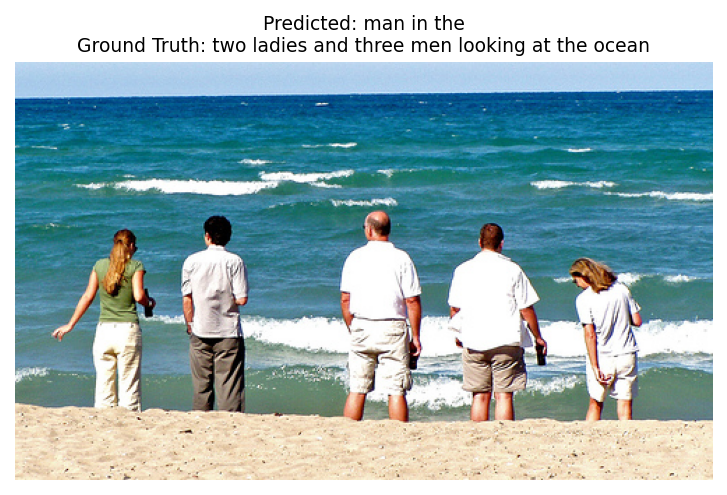
\includegraphics[width=0.78\textwidth]{baseline_example.png}
  \caption{Esempio rappresentativo della configurazione baseline.}
\end{figure}

Nel caso della baseline, la caption prodotta tende a essere sintatticamente corretta ma relativamente generica. Questo comportamento è tipico di modelli che apprendono strutture frasali robuste ma non sono ancora sufficientemente sensibili ai dettagli distintivi dell'immagine. Dal punto di vista metodologico, la baseline dimostra che la pipeline CNN--LSTM è funzionale, ma anche che l'estrattore congelato limita la specificità della descrizione.

\section{Esempio di fine-tuning}

\begin{figure}[H]
  \centering
  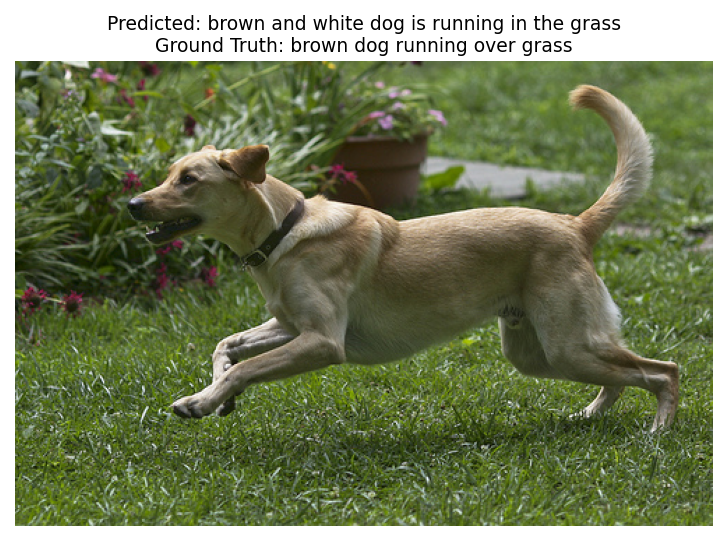
\includegraphics[width=0.78\textwidth]{finetune_example.png}
  \caption{Esempio qualitativamente riuscito della configurazione con fine-tuning della CNN.}
\end{figure}

La configurazione con fine-tuning mostra una migliore capacità di catturare il soggetto principale e l'azione in corso. La differenza non consiste tanto nella lunghezza della frase, quanto nella sua maggiore pertinenza. Questo è perfettamente coerente con il miglioramento osservato nei punteggi BLEU: non si tratta di un guadagno casuale, ma di un segnale che l'encoder visivo adattato al task produce feature più utili per il decoder.

\section{Failure case}

\begin{figure}[H]
  \centering
  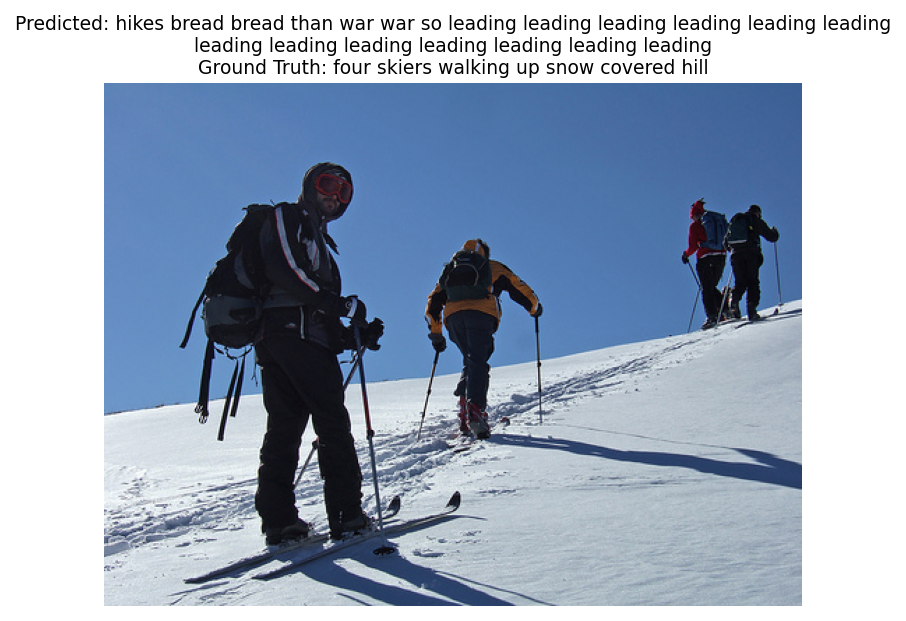
\includegraphics[width=0.78\textwidth]{failure_case.png}
  \caption{Caso di fallimento utile per discutere i limiti del modello.}
\end{figure}

Il \emph{failure case} selezionato è forse ancora più informativo degli esempi positivi. In esso il modello produce una descrizione rumorosa o ripetitiva, evidenziando due limiti tipici delle architetture ricorrenti di questo tipo: la tendenza a collassare su sequenze lessicali altamente frequenti e la difficoltà nel rappresentare in modo affidabile configurazioni visive meno comuni. L'inclusione di esempi di fallimento è fondamentale in una narrativa accademica seria, perché impedisce di trasformare la sezione qualitativa in una semplice vetrina di casi favorevoli.

\chapter{Discussione dei Limiti e Prospettive Future}

\section{Limiti empirici emersi}

I risultati quantitativi e qualitativi consentono di identificare con chiarezza alcuni limiti del sistema. Il primo è la tendenza alla genericità descrittiva in assenza di un encoder adattato al dominio. Il secondo è la sensibilità a errori autoregressivi, che si manifesta nella degradazione osservata quando si rimuove lo scheduled sampling. Il terzo è la difficoltà nel mantenere ricchezza lessicale e robustezza al tempo stesso, evidenziata dal calo di BLEU dovuto alla rimozione del label smoothing.

Un ulteriore limite riguarda il rapporto tra validation loss e qualità finale delle caption. I risultati mostrano che la configurazione migliore in termini di BLEU non è necessariamente quella con la loss finale più bassa. Questo suggerisce che, in un progetto di captioning, la loss deve essere interpretata come segnale utile ma non sufficiente: è necessario affiancarle una valutazione testuale effettiva.

\section{Limiti strutturali dell'architettura}

La combinazione CNN--LSTM è coerente con la traccia e pedagogicamente molto utile, ma non rappresenta più lo stato dell'arte nel captioning. La mancanza di un meccanismo di attenzione multimodale esplicito, l'uso di greedy decoding e l'assenza di tokenizzazione subword limitano la capacità del sistema di produrre caption ricche, specifiche e robuste a lessico raro. Tuttavia, proprio questa semplicità rende il progetto leggibile e sperimentalmente controllabile.

\section{Sviluppi futuri realistici}

Gli sviluppi più naturali del lavoro sono almeno quattro. In primo luogo, introdurre un decoder più espressivo o un meccanismo di attenzione esplicita tra feature visive e stati linguistici. In secondo luogo, sostituire il vocabolario word-level con una tokenizzazione subword, così da ridurre l'impatto degli OOV. In terzo luogo, adottare strategie di decoding più ricche, come beam search, per migliorare la qualità finale delle caption senza modificare radicalmente l'architettura. Infine, ampliare la valutazione includendo metriche aggiuntive come CIDEr o SPICE, più specifiche per il captioning rispetto al solo BLEU.

\chapter{Conclusioni}

Il progetto ha prodotto un sistema completo di image captioning basato su CNN--LSTM, corredato da pipeline dati, configurazioni di training, salvataggio checkpoint, valutazione quantitativa e analisi qualitativa. La revisione documentale presentata in questo report ha avuto il compito di riallineare la descrizione teorica e implementativa agli esperimenti realmente eseguiti, evitando sia l'eccesso di generalità sia la sovrastima dei risultati.

Dal punto di vista sperimentale, le conclusioni sono nette. Lo scheduled sampling e il label smoothing contribuiscono positivamente alla qualità linguistica del decoder, mentre il fine-tuning della CNN costituisce la modifica che produce il miglior miglioramento complessivo. Dal punto di vista metodologico, il progetto dimostra anche un principio più generale: in compiti generativi multimodali, la sola loss non basta per giudicare la bontà del modello, e deve essere sempre integrata con metriche esterne e analisi qualitative.

Nel suo insieme, il lavoro risulta quindi solido non perché raggiunga valori assoluti elevati rispetto allo stato dell'arte, ma perché costruisce una pipeline coerente, riproducibile e criticamente analizzata. Questo è precisamente il tipo di risultato che un progetto accademico ben documentato dovrebbe offrire.

\appendix

\chapter{Fondamenti Teorici di Supporto}

Questa appendice raccoglie i richiami teorici essenziali sui principali concetti impiegati nel progetto, con particolare riferimento ai fondamenti del deep learning, alle reti neurali convoluzionali e alle LSTM. La loro collocazione in appendice risponde a una scelta di organizzazione del testo: nel corpo centrale si è privilegiata la descrizione della pipeline sviluppata, del protocollo sperimentale e dei risultati ottenuti, mentre il quadro teorico generale viene qui mantenuto come supporto alla lettura.

\section{Perché mantenere il materiale teorico}

Il richiamo teorico conserva una funzione importante all'interno dell'elaborato, poiché consente di inquadrare correttamente le scelte architetturali adottate e la logica delle procedure di addestramento. In particolare, i concetti relativi alla rappresentazione delle feature visive, alla modellazione sequenziale e alla stabilizzazione del training costituiscono il presupposto necessario per interpretare in modo rigoroso il comportamento del modello CNN--LSTM discusso nei capitoli precedenti.

\chapter{Struttura del Repository e Riproducibilità}

\section{File principali del progetto}

La versione finale del repository ruota attorno ai seguenti file:
\begin{itemize}[leftmargin=*]
  \item \texttt{src/prepare\_data.py}: genera vocabolario e split a partire dai file originali di Flickr8k;
  \item \texttt{src/dataset.py}: definisce il dataset e il caricamento delle coppie immagine-caption;
  \item \texttt{src/model.py}: implementa encoder convoluzionale e decoder LSTM;
  \item \texttt{src/train.py}: esegue il training, gestisce checkpoint e validazione;
  \item \texttt{src/eval.py}: calcola le metriche BLEU sul test set;
  \item \texttt{src/visualize.py}: genera esempi qualitativi a partire dal modello addestrato.
\end{itemize}

\section{Configurazioni e comandi utilizzati}

Le run finali sono state eseguite con i file di configurazione in \texttt{configs/}. I comandi principali sono stati:

\begin{verbatim}
python src/prepare_data.py
python -u src/train.py --config configs/baseline_cpu.yml
python -u src/train.py --config configs/ablation_no_scheduled_sampling_cpu.yml
python -u src/train.py --config configs/ablation_no_label_smoothing_cpu.yml
python -u src/train.py --config configs/ablation_finetune_cpu.yml
\end{verbatim}

Per l'evaluation:

\begin{verbatim}
python -u src/eval.py --images_dir data/Flickr8k_Dataset \
  --captions_json data/Flickr8k_text/test_captions.json \
  --vocab_path data/vocab.json \
  --weights checkpoints/<experiment>/model_best.pt
\end{verbatim}

\section{Artefatti finali}

Gli output principali prodotti e utilizzati nel report sono:
\begin{itemize}[leftmargin=*]
  \item \texttt{results/metrics\_summary.csv};
  \item \texttt{results/experiment\_summary.csv};
  \item checkpoint in \texttt{checkpoints/};
  \item log in \texttt{logs/};
  \item figure qualitative in \texttt{figures/} e \texttt{docs/selected\_figures/}.
\end{itemize}

\end{document}
